% -- Document configuration
\documentclass{article}

% -- Input and language settings
% \usepackage[utf8]{inputenc}
\usepackage[spanish]{babel}
\decimalpoint                             % From babel package to use points instead of commas in decimals

% -- Page and line settings
\usepackage{geometry}
\geometry{letterpaper, 
    % margin=2cm, 
    left=3cm, right=3cm,
    top=1.2cm, bottom=1.2cm,
    includefoot, 
    includehead}
\renewcommand{\baselinestretch}{1.2}

% -- Required packages
\usepackage{xcolor}
\usepackage[many]{tcolorbox}
\usepackage{mathtools,amsfonts,amsmath}     % Loads amsmath if not already loaded
\allowdisplaybreaks                         % To allow page breaks if equations are too long
\usepackage[parfill]{parskip}               % No indent and separation lines for paragraphs
\usepackage{cancel}                         % To cancel math terms
\usepackage[shortlabels]{enumitem}          % To handle enumerations
\usepackage{tikz}
\usetikzlibrary{automata, arrows.meta, positioning}
\usepackage[mode=buildnew]{standalone}      % To import figures in standalone files
\usepackage[hidelinks]{hyperref}
\usepackage[spanish]{cleveref}              % To use autocompleted reference labels, language must be change as in babel package
\usepackage{caption}                        % Caption and subcaption to allow subfigures
\usepackage{subcaption}
\usepackage{float}                          % To specify the location of figures
\usepackage{multicol}                       % To use multicolumns
\usepackage[bottom]{footmisc}               % To locate footnotes at the bottom

% -- Title and heading settings
\usepackage{titling}
\usepackage{fancyhdr}
\pagestyle{fancy}

% -- Code and code formatting
\usepackage{minted}                         % To insert code
\usemintedstyle[julia]{gruvbox-light}       % Code theme and language
\definecolor{bg}{rgb}{0.98, 0.97, 0.88}     % Code block background

\usepackage{fontspec}                       % To allow the use of monospace fonts
\setmonofont{JuliaMono}[Path=./codefonts/, Extension=.ttf, UprightFont=*-Regular, ItalicFont=*-RegularItalic, Scale=0.75]

\usepackage{fancyvrb}                       % To change line number font
\renewcommand{\theFancyVerbLine}{\textcolor{gray}{\footnotesize\texttt{\arabic{FancyVerbLine}}}}

\definecolor{light-gray}{gray}{0.95}        % Color, box and style to show small code thingys inside normal text
\newcommand{\code}[1]{\colorbox{light-gray}{\texttt{#1}}}

% -- Bilbiography preferences
\usepackage[square,numbers]{natbib}
\bibliographystyle{unsrt}

% -- Footnotes without numbering
\newcommand\nnfootnote[1]{%
  \begin{NoHyper}
  \renewcommand\thefootnote{}\footnote{#1}%
  \addtocounter{footnote}{-1}%
  \end{NoHyper}
}

% -- Theorems
\newtheorem{theorem}{Theorem}

\lhead{\theinstitution\ -- \thedepartment}
\chead{}
\rhead{Programación para la IA\ -- \thetitle}
\lfoot{}
\cfoot{\thepage}
\rfoot{}

% -- Problem solution
\newenvironment{solution}
{\begin{quote}
\textbf{Solución:}\medskip

}
{

\hfill\rule{0.5\textwidth}{0.5pt}
\end{quote}}

% -- Equation result
\newcommand{\result}[1]
{
\tcbhighmath[colframe=white, colback=gray!15, sharp corners]
{#1}
}

% -- Function definitions
\newcommand{\dprod}[2]{{#1} \cdot {#2}}
\newcommand{\txtgray}[1]{\textcolor{gray}{#1}}

% -- Author information
\title{Actividad 5}
\author{Leonardo Flores Torres}
\newcommand\theinstitution{Universidad Veracruzana}
\newcommand\thedepartment{Inteligencia Artificial}
\newcommand\thecourse{Programación para la Inteligencia Artificial}

% -- Paths
% \newcommand\codelists{../programs/lists.rkt}

% Remove red color boxes of "syntax errors" in minted
\AtBeginEnvironment{minted}{%
  \renewcommand{\fcolorbox}[4][]{#4}}

% -- Document
\begin{document}

\thispagestyle{empty}

%Title
\begin{center}
\textsc{\theinstitution}\\[2mm]

\thedepartment

\rule{0.6\textwidth}{0.5pt}\\[2mm]

\thecourse \\[4mm]

{\Large \textbf{\thetitle}}\\[2mm]

\theauthor \\[2mm]

{\small \today}
\end{center}
\medskip

% -- 
\vspace{1cm}

\begin{enumerate}
    \item Ajuste de distribuciones de probabilidad a datos de entrenamiento y la distribución predictiva para una distribución Gaussiana unidimensional. Defina $N > 10$ puntos aleatorios extraídos de una distribución gaussiana $\text{G}_{x}(\mu_0, \sigma_0)$, con $\mu_0 = 5$ y $\sigma_0 = 1.5$, $\text{RandomG}_{x}(\sigma_0, \mu_0)$.
    \begin{solution}
        Una distribución normal univariada $\text{Norm}_{x}[\sigma, \mu]$ está dada por
        \begin{equation}
            \text{Norm}_{x}[\sigma, \mu] = \frac{1}{\sqrt{2 \pi \sigma^2}} \exp\left[- \frac{1}{2} \frac{(x - \mu)^2}{\sigma^2}\right],
        \end{equation}
        donde $\mu$ es la media y $\sigma$ es la desviación estándar. Se generó una distribución normal univariada centrada en $\mu_0  = 5$ con desviación estándar $\sigma_0 = 1.5$, como se muestra en la \cref{fig:original}, con dominio $D_0 : \{x\ |\ x \in \left[\mu_0 - 3.5 \sigma_0,\ \mu_0 + 3.5 \sigma_0\right]\}$. De esta distribución normal se realizó un muestreo para extraer un número $N = 30$ de datos los cuales son el conjunto de entrenamiento $\{x_i\}_{i=1}^{30}$ usado en el resto de los incisos a responder en esta actividad.
        \begin{figure}[ht!]
            \centering
            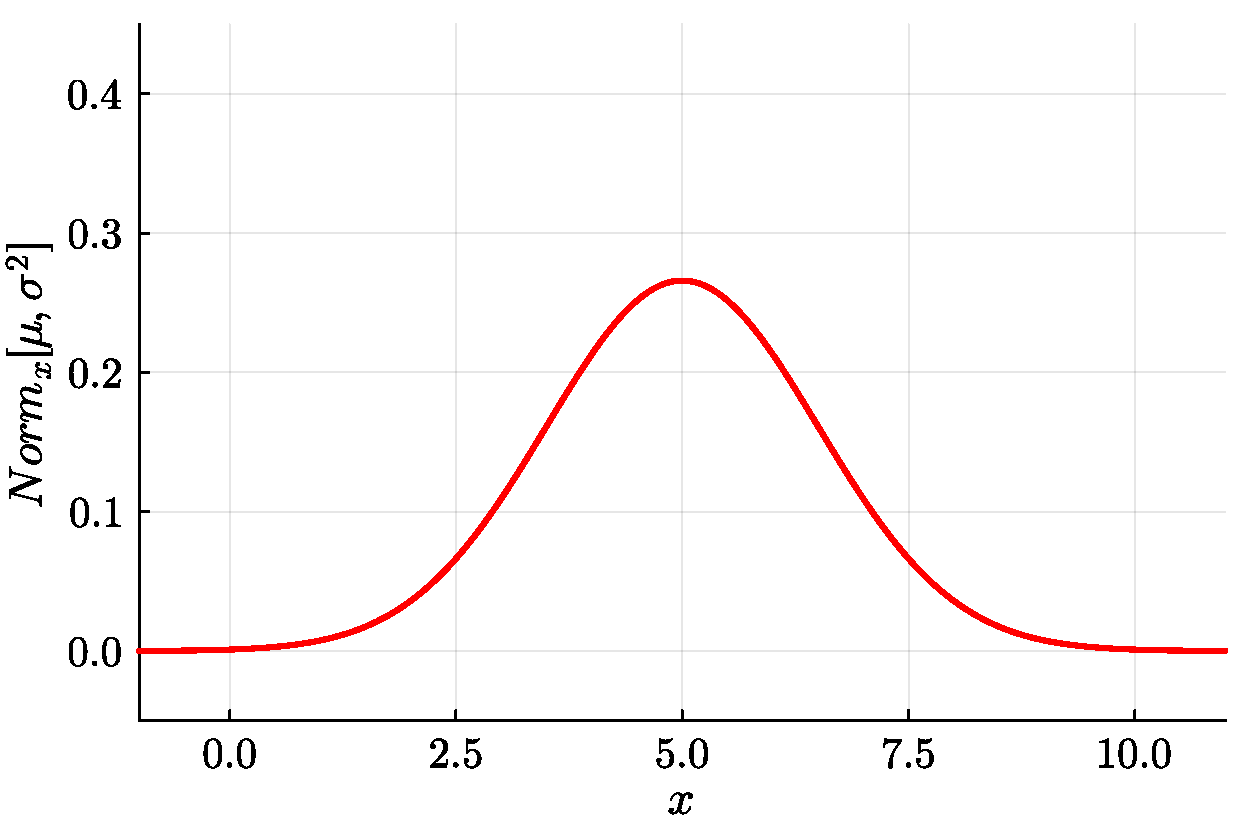
\includegraphics[scale=0.4]{../figures/original.pdf}
            \caption{Distribución gaussiana de probabilidad usada para extrar los datos de entrenamiento.}
            \label{fig:original}
        \end{figure}
        
        Solamente para clarificar, los parámetros que maximizan la verosimilitud $\{\hat{\mu}, \hat{\sigma}\}$ se encuentran al computar las derivadas e igualando a cero para encontrar un máximo, respecto a cada uno de los parámetros $\{\mu, \sigma\}$, del producto de las verosimilitudes individuales para cada uno de los puntos del conjunto muestreal $\{x_i\}_{i=1}^{N}$. Como se está usando una distribución normal univariada se tiene que la verosimilitud es igual a
        \begin{equation}
            \text{Pr}(x_{1 \ldots N} | \mu, \sigma^2) = \prod\limits_{i=1}^{N}\text{Norm}_{x_i} \left[\mu, \sigma^2\right].
        \end{equation}
        Después de encontrar las derivadas respecto a cada uno de los parámetros e igualando a cero se obtiene que los parámetros que maximizan la verosimilitud son
        \begin{align}
            \hat{\mu} & = \frac{1}{N} \sum\limits_{i=1}^{N} x_i\ ,\\
            \hat{\sigma}^2 & = \frac{1}{N} \sum\limits_{i=1}^{N} \left(x_i - \hat{\mu}\right)^2\ .
        \end{align}
        
        Para generar estos datos se definen los parámetros iniciales \code{$\mu_0$} y \code{$\sigma_0$}, se define el dominio en \code{x0}, y el muestreo se computa en \code{xsample}. También se computan los valores de la gaussiana en el dominio, i.e., $\text{G}_{x_0}(\mu_0, \sigma_0)$. Es importante mencionar que el dominio será el mismo en todas las demás distribuciones que se generen, esto quiere decir $D_i = D_0$ para $i = 1, 2, 3$ donde $i$ denota el conjunto de condiciones $\{\mu_i,\ \sigma_i\}$ mencionadas en el segundo inciso de la actividad.
        \begin{minted}[
            frame=none,
            autogobble,
            obeytabs=false,
            breaklines,
            tabsize=4,
            linenos=true,
            % numbersep=-10pt,
            baselinestretch=1,
            firstnumber=1,
            bgcolor=bg!70,
            ]{julia}
            julia> using Revise, NormalDist; nd = NormalDist;
            julia> begin
                   # Parametros iniciales de la gaussiana
                   μ0 = 5
                   σ0 = 1.5
                   # Dominio de la gaussiana original
                   x0 = range(μ0 - 4 * σ0, μ0 + 4 * σ0, 2000)
                   # Evaluacion de la gaussiana en el dominio G(x0)
                   w0 = nd.normalDist(x0, μ0, σ0)
                   # Numero de puntos para muestreo
                   npts = 30
                   # Muestreo de puntos
                   xsample = nd.randomSample(x0, w0, npts)
                   # Grafica de la gaussiana
                   fig = nd.plotNormal(x0, w0)
                   end
        \end{minted}
        Nótese que en ningún momento se ha mencionado que es necesario restringir el conjunto de entrenamiento a valores únicos, por lo que está permitido tener puntos repetidos dentro del conjunto aleatorio de entrenamiento $\{x_i\}_{i}^{30}$.
    \end{solution}
    \item Grafique 3 figuras como la lámina 16 del Prince, diapositiva 4, donde se muestren los $N$ puntos, y los valores del likelihood para 3 Gaussianas considerando
    \begin{enumerate}
        \item $\mu_1 = 3$, $\sigma_1 = 1$,
        \item $\mu_2 = 6$, $\sigma_2 = 1.6$,
        \item $\mu_3 = 5.1$, $\sigma_3 = 1.4$.
    \end{enumerate}
    Grafique las Gaussianas sobre los puntos de entrenamiento y su ordenada para cada Gaussiana, $\text{Gauss}_{x}(\mu_i, \sigma_i)$.
    \begin{solution}
        Un ejemplo de como se computaron todas las distribuciones se muestra a continuación:
        \begin{minted}[
            frame=none,
            autogobble,
            obeytabs=false,
            breaklines,
            tabsize=4,
            linenos=true,
            % numbersep=-10pt,
            baselinestretch=1,
            firstnumber=last,
            bgcolor=bg!70,
            mathescape,
            ]{julia}
            julia> begin
                   # Parametros para el i-esimo caso
                   μi = 6       # parametro μi $\label{line:mui}$
                   σi = 1.6     # parametro σi $\label{line:sigmai}$
                   # Evaluacion de la i-esima gaussiana con nuevos parametros sobre el conjunto de datos muestreados
                   wsample = nd.normalDist(xsample, μi, σi)
                   # Computo de la i-esima gaussiana con nuevos parametros
                   wi = nd.normalDist(x0, μi, σi)
                   # Likelihood de los datos xsample respecto a los i-esimos parametros
                   lh = nd.likelihood(xsample, μi, σi)
                   # Grafica de la i-esima gaussiana con los datos muestreados
                   fig = nd.plotGuess(xsample, wsample, x0, wi, lh, μi, σi; maxlh = false)
                   end
        \end{minted}
        Las gaussianas obtenidas con sus respectivos parámetros se muestran en la \cref{fig:gaussianas}, donde también se incluyó la gráfica para la gaussiana con los parámetros que maximizan la verosimilitud $\{\hat{\mu},\ \hat{\sigma}\}$. Además, cada gráfica incluye su verosimilitud dependiendo de sus parámetros $Pr(x_{1 \ldots 30} |\ \mu_i,\ \sigma_{i}^2)$. Para el caso de $\{\hat{\mu},\ \hat{\sigma}\}$ sólamente se realizaron las siguientes asignaciones \code{μi = nd.maxμ(xsample)} y \code{σi = nd.maxσ(xsample)} en las lineas \ref{line:mui} y \ref{line:sigmai}, y se cambia el parámetro \code{maxlh = true} de la función donde se genera la gráfica para decir al programa que cambie el título de la gráfica.
        \begin{figure}[H]
            \centering
            \begin{subfigure}{\textwidth}
                \centering
                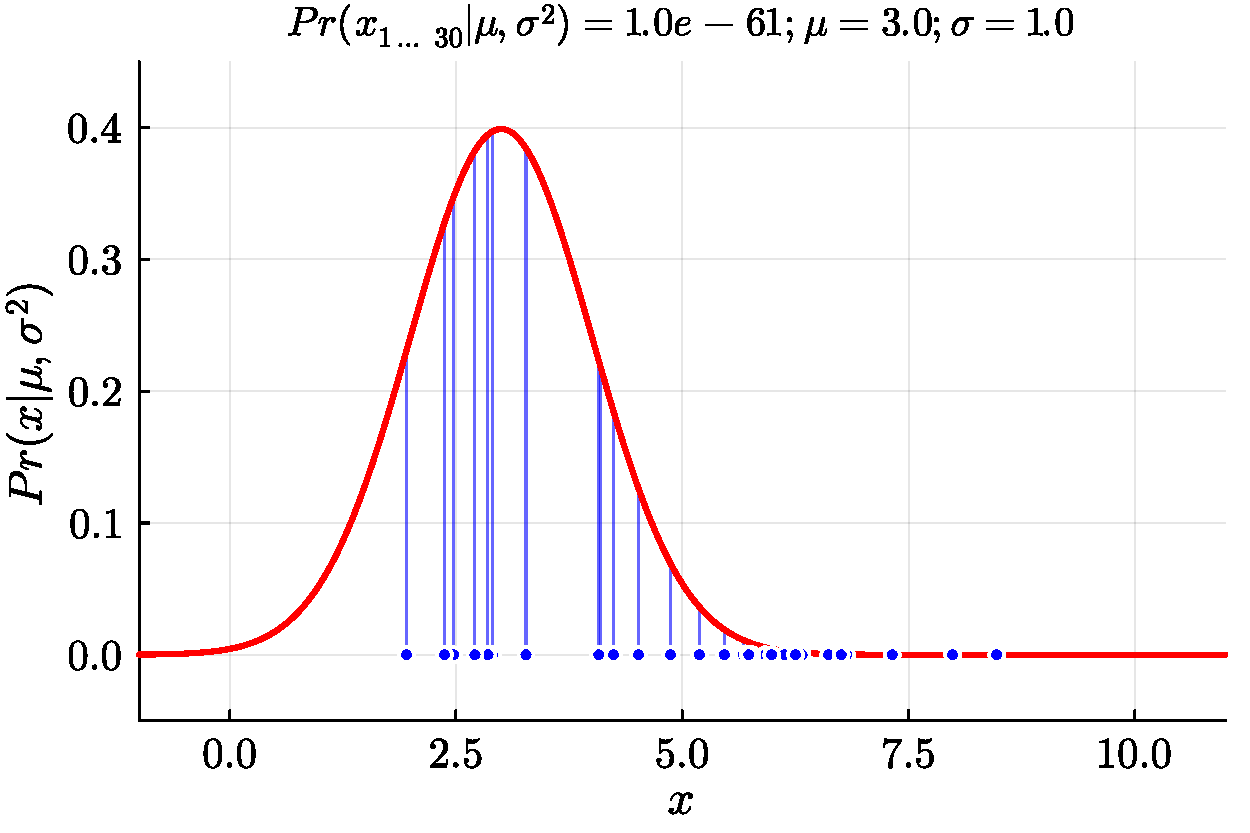
\includegraphics[scale=0.4]{../figures/dist_1.pdf}
                \caption{Distribución $G_{x}(\mu_1, \sigma_1)$ para los parámetros $\mu_1 = 3$, $\sigma_1 = 1$.}
                \label{fig:gaussiana_1}
            \end{subfigure}
        \end{figure}
        \begin{figure}[H]
            \ContinuedFloat
            \begin{subfigure}{\textwidth}
                \centering
                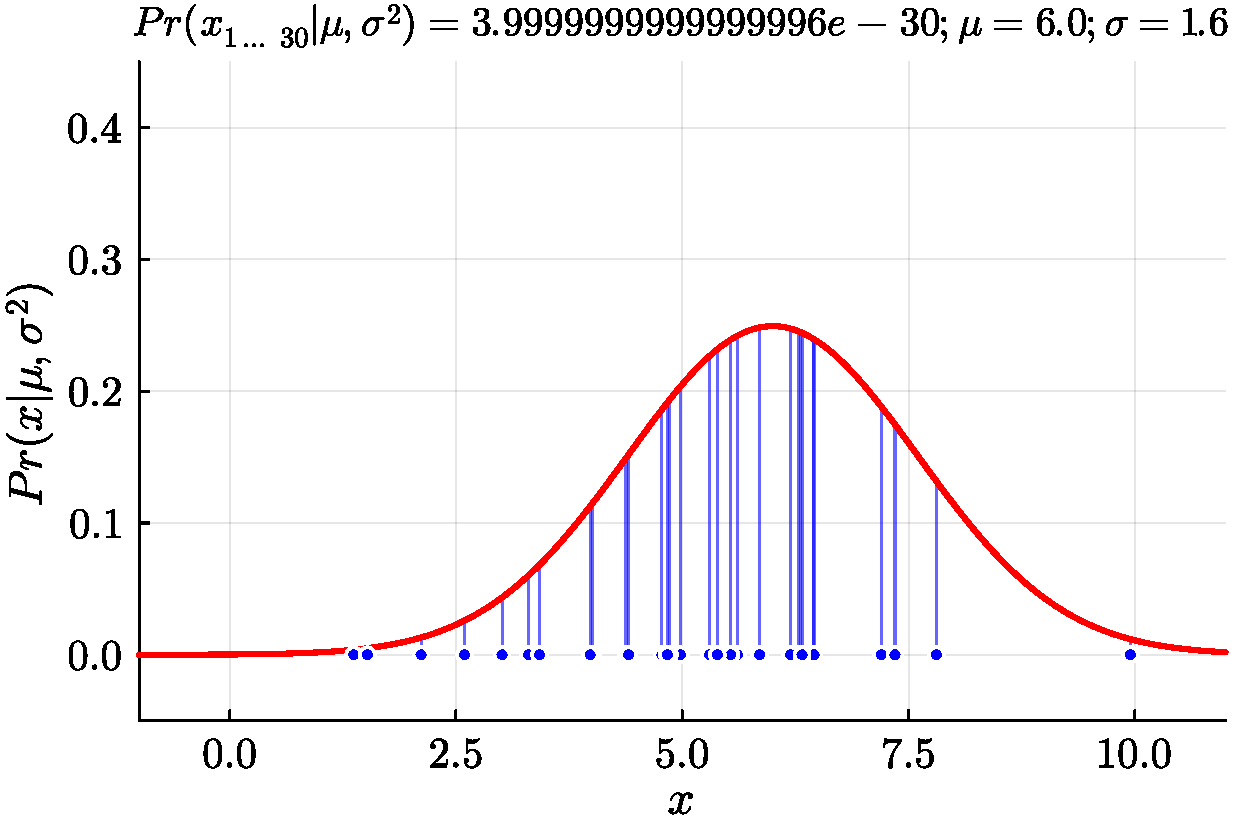
\includegraphics[scale=0.4]{../figures/dist_2.pdf}
                \caption{Distribución $G_{x}(\mu_2, \sigma_2)$ para los parámetros $\mu_2 = 6$, $\sigma_2 = 1.6$.}
                \label{fig:gaussiana_2}
            \end{subfigure}
        \end{figure}
        \begin{figure}[H]
            \ContinuedFloat
            \begin{subfigure}{\textwidth}
                \centering
                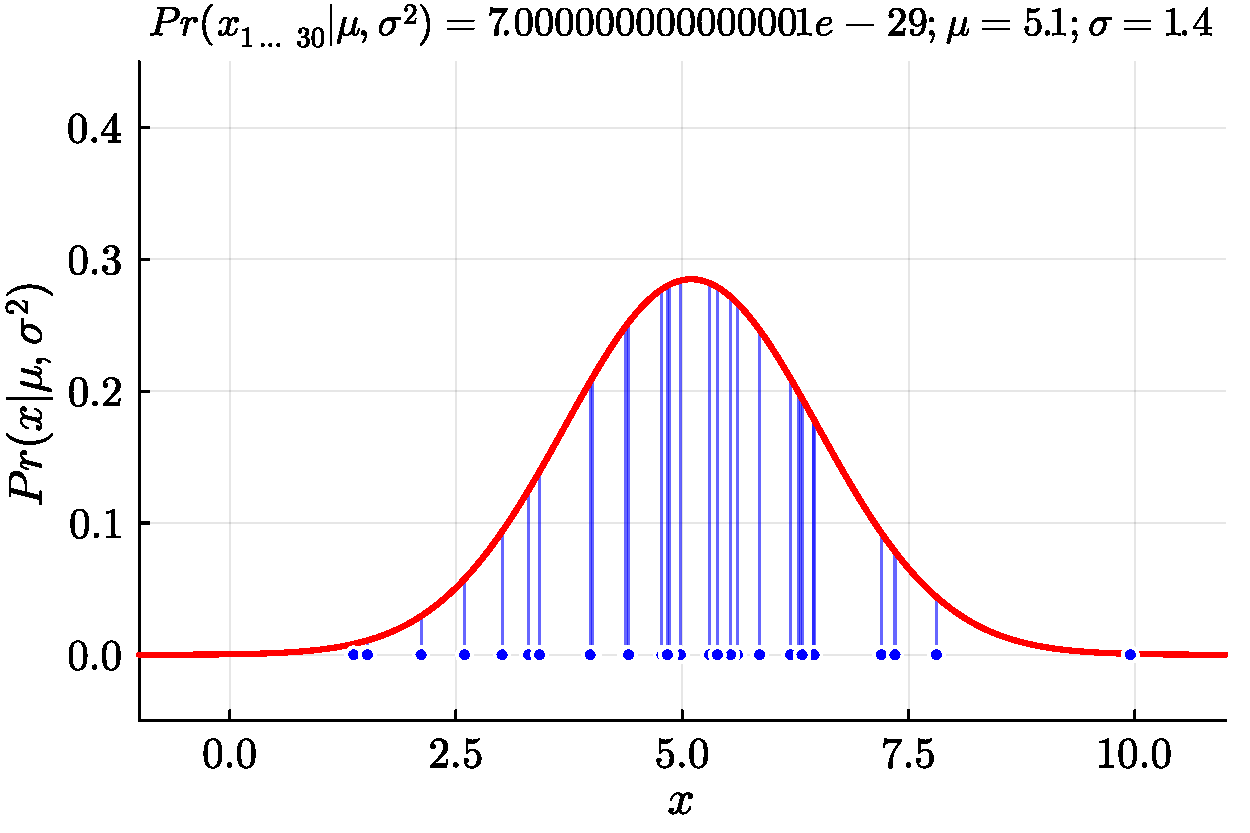
\includegraphics[scale=0.4]{../figures/dist_3.pdf}
                \caption{Distribución $G_{x}(\mu_3, \sigma_3)$ para los parámetros $\mu_3 = 5.1$, $\sigma_3 = 1.4$.}
                \label{fig:gaussiana_3}
            \end{subfigure}
        \end{figure}
        \begin{figure}[H]
            \ContinuedFloat
            \begin{subfigure}{\textwidth}
                \centering
                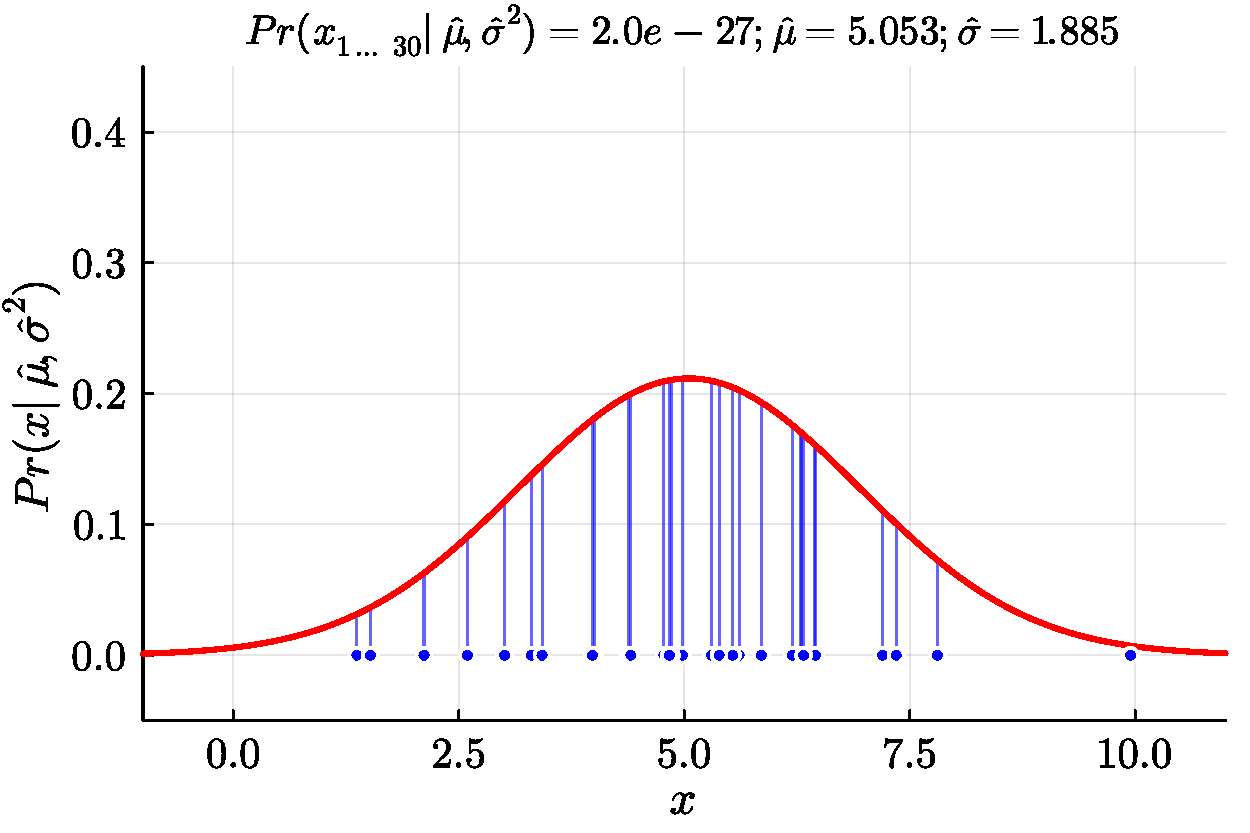
\includegraphics[scale=0.4]{../figures/dist_max.pdf}
                \caption{Distribución $G_{x}(\hat{\mu}, \hat{\sigma})$ para los parámetros que maximizan el likelihood, $\hat{\mu}$, $\hat{\sigma}$.}
                \label{fig:gaussiana_max}
            \end{subfigure}
            \caption{Gráficas de las gaussianas requeridas para el segundo punto de la actividad con sus respectivos parámetros.}
            \label{fig:gaussianas}
        \end{figure}

        Nótese que para el conjunto de puntos muestreados $\{x_i\}_{i=1}^{30}$ se obtiene un buen valor para la verosimilitud, con parámetros $\{\hat{\mu} = 5.053,\ \hat{\sigma} = 1.885\}$.

    \end{solution}
    \item Genere el mapa térmico de las probabilidades considerando $\mu \in \left[2.5, 6.5\right]$, y $\sigma \in \left[0, 2\right]$, dividiendo ambos intervalos en 10 partes. Coloque un marcador en el punto de máxima verosimilitud.
    \item Calcule, usando el método de Maximum Likelihood, los parámetros $\hat{\mu}$ y $\hat{\sigma}^2$ que tanto coincide con el mapa térmico.
    \begin{solution}
        Los incisos 3 y 4 se resolvieron de manera conjunta ya que al añadir un marcador en el mapa de calor que indique donde se encuentra el punto de máxima verosimilitud este se tuvo que haber computado de antemano. Me tomé la libertad de cambiar el número de divisiones a 30 en que se subdividen los intervalos para $\mu$ y $\sigma$. La instrucción escrita en \code{julia} que genera el mapa de calor se muestra a continuación:
        \begin{minted}[
            frame=none,
            autogobble,
            obeytabs=false,
            breaklines,
            tabsize=4,
            linenos=true,
            % numbersep=-10pt,
            baselinestretch=1,
            firstnumber=last,
            bgcolor=bg!70,
            ]{julia}
            julia> begin 
                   # Numero de particiones para los intervalos de μ y σ
                   partitions = 30
                   # Intervalos de μ y σ
                   μint = (2.5, 6.5)
                   σint = (0, 2)
                   # Deltas de μ y σ
                   dμ = (μint[2] - μint[1]) / partitions
                   dσ = (σint[2] - σint[1]) / partitions
                   # Dominios de μ y σ
                   μrange = range(μint[1] + dμ/2, μint[2] - dμ/2, partitions)
                   σrange = range(σint[1] + dσ/2, σint[2] - dσ/2, partitions)
                   # Mallado para obtener un espacio bidimensional
                   (μmesh, σmesh) = nd.ndgrid(μrange, σrange)
                   # Valores del likelihood en el mallado
                   lhmesh = nd.likelihood.(Ref(xsample), μmesh, σmesh)
                   # Parametros que maximizan el likelihood y el likelihood maximo
                   μmax = nd.maxμ(xsample)
                   σmax = nd.maxσ(xsample)
                   lhmax = nd.likelihood(xsample, μmax, σmax)
                   # Grafica del mallado
                   fig = nd.plotHeat([3, 6, 5.1], [1, 1.6, 1.4], μmax, σmax, μrange, σrange, lhmesh, npts)
                   end
        \end{minted}
        El mapa de calor se muestra en la \cref{fig:heatmap}. El punto de máxima verosimilitud con parámetros $\{\hat{\mu}, \hat{\sigma}\}$ está marcado con una estrella de color cyan, mientras que los demás puntos marcados con círculos color magenta corresponden a las verosimilitudes con sus conjuntos respectivos de parámetros $\{\mu_i, \sigma_i\}$.
        \begin{figure}[ht!]
            \centering
            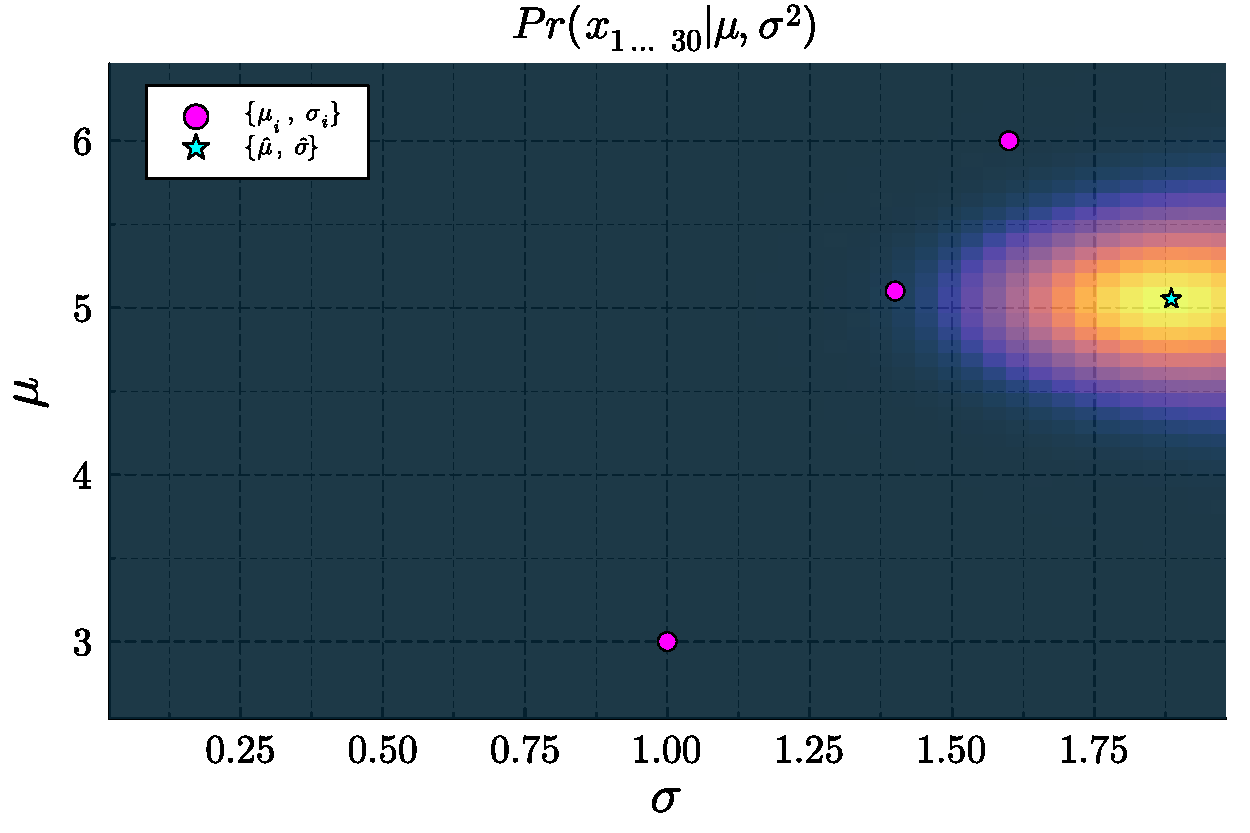
\includegraphics[scale=0.5]{../figures/heatmap.pdf}
            \caption{Mapa de calor incluyendo las verosimilitudes de sus respectivos parámetros.}
            \label{fig:heatmap}
        \end{figure}
        Los valores para las verosimilitudes de cada uno de los casos se puede observar en el título de las \cref{fig:gaussiana_1,fig:gaussiana_2,fig:gaussiana_3,fig:gaussiana_max} con sus respectivos parámetros. El muestreo no es perfecto, mientras más puntos se obtengan para el muestreo mejor será la aproximación para la máxima verosimilitud. Aún así, mientras computaba las distribuciones gaussianas $G_{x}(\mu_i, \sigma_i)$ me encontraba seguido con el caso de que el la máxima verosimilitud era menor que la verosimilitud para el caso $\{\mu_3 = 5.1, \sigma_3 = 1.4\}$. Atribuyo este comportamiento como resultado del muestreo, pero la máxima verosimilitud siempre parecía encontrarse en el centro del elipsoide del mapa de calor.
    \end{solution}
\end{enumerate}

\section*{Apéndice}
\inputminted[
    frame=none,
    autogobble,
    obeytabs=false,
    breaklines,
    tabsize=4,
    linenos=true,
    % numbersep=-10pt,
    baselinestretch=1,
    firstnumber=1,
    bgcolor=bg!70,]{julia}{\codepath}

\nocite{*} % to call all references even if they are not cited in the text
\bibliography{references.bib}

\end{document}